
\section{Spectral analysis} \label{sec:Spectra}

The turbulent fluctuations are due to the interactions of a wide range of coherent structures of different sizes. Each of these structures will have a characteristic length and energy content. Depending on the approach used to decompose the energy content of the Reynolds-stress components in space/time we can have different types of representations.
The spectral analysis used here is based on a Fourier decomposition of the spanwise two-point correlations. The velocity correlation between two points along the spanwise direction provides an idea of lengths at which the fluctuations are highly correlated, and this gives an indication of the presence of a certain structure or pattern. In a multi-scale phenomenon such as turbulence at high Reynolds numbers, the two-point correlations will contain a mix of all the different scales and it will be difficult to obtain meaningful information from it. 
Since the spanwise direction is periodic, a Fourier decomposition of the two-point correlation is possible, and the result is a spectral decomposition of the energy content in different wavenumbers $k_z$ associated with their corresponding wavelengths $\lambda_z=2\pi/k_z$. 
In the next sections we show the premultiplied power-spectral density of the different Reynolds-stress components at matched values of $\Rey_{\tau}=500, 1000,1500,2000$. For reference, an additional contour has been added in gray for the maximum $\Rey_{\tau}=2386$ in the ZPG simulation.

%-------------------- Spec1D APG-ZPG ------------------------------------------------------------------------
\subsection{One-dimensional power-spectral density in z}

\begin{figure}
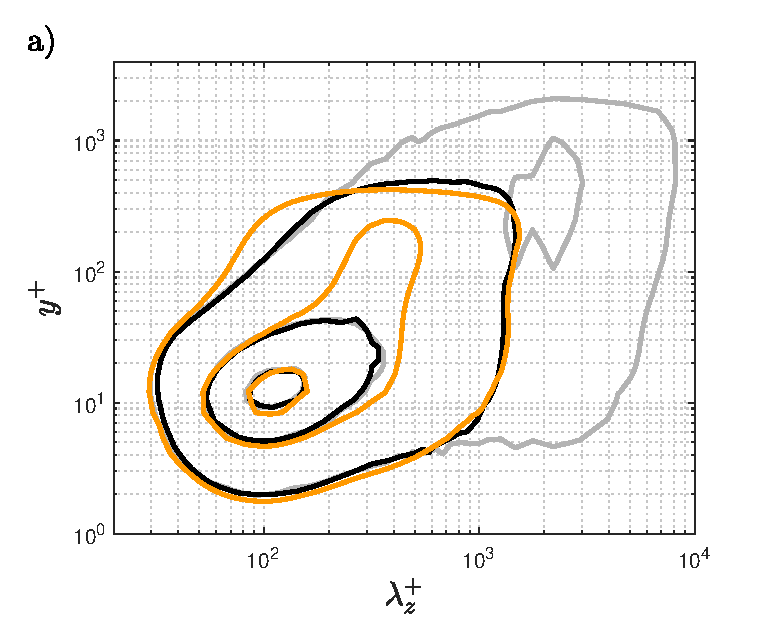
\includegraphics[width=0.49\textwidth]{fig11a.eps}
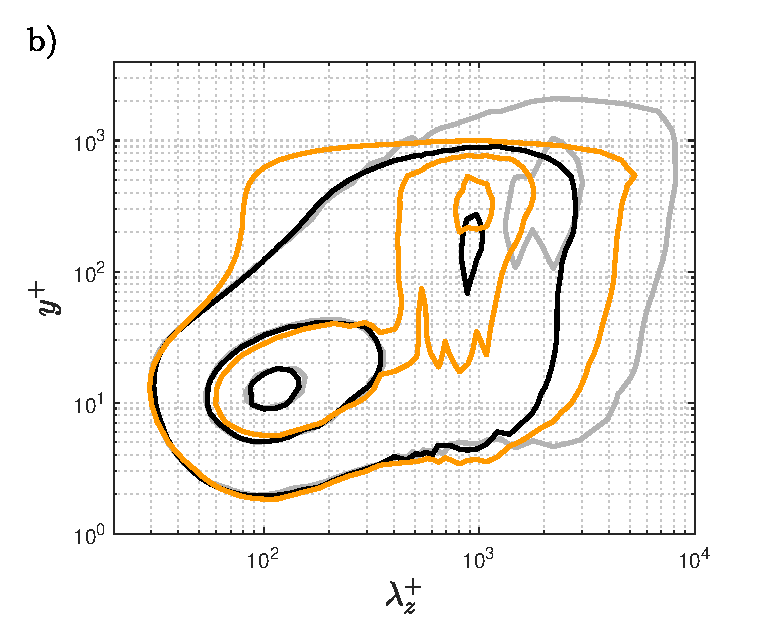
\includegraphics[width=0.49\textwidth]{fig11b.eps}
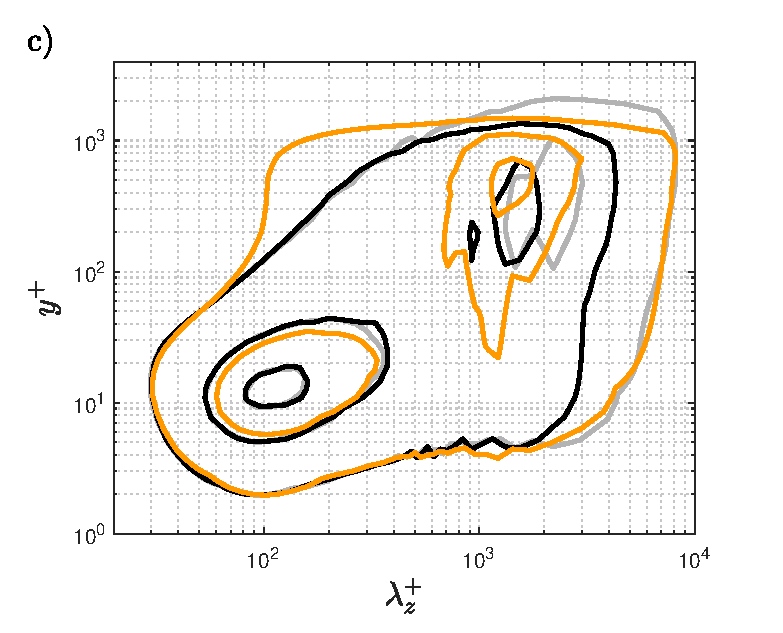
\includegraphics[width=0.49\textwidth]{fig11c.eps}
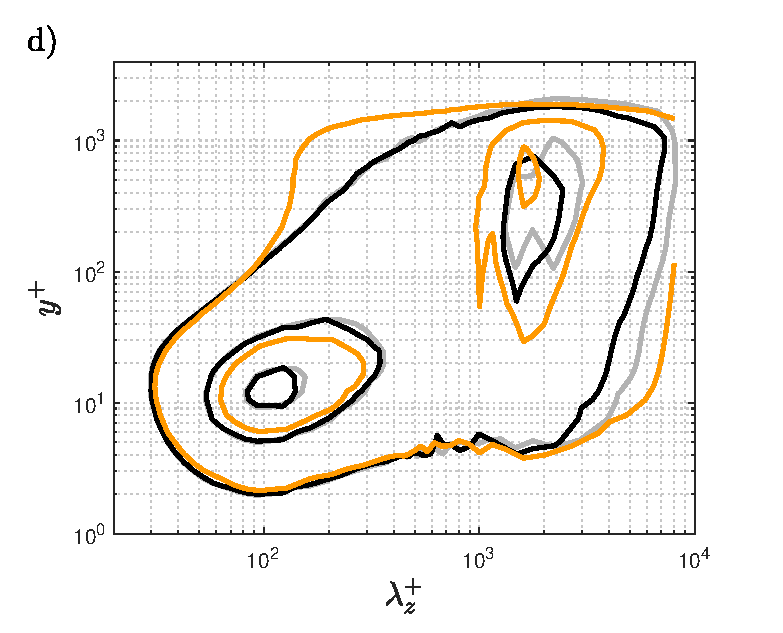
\includegraphics[width=0.49\textwidth]{fig11d.eps}
  \caption{Premultiplied spanwise power-spectral density $k_z |\phi_{uu}|$ scaled with the local maximum for the b1.4 and ZPG cases at matched $\Rey_{\tau}$. Contours taken at $10\%$, $50\%$, $90\%$ of the maximum value. Reference contour in gray colour: ZPG at $Re_{\tau}=2386$. Contours with (\protect\blackline) for ZPG and (\protect\orangeline) for b1.4. (Top-left) $Re_{\tau}=500$, (top-right) $Re_{\tau}=1000$, (bottom-left) $Re_{\tau}=1500$, (bottom-right) $Re_{\tau}=2000$.}
\label{fig:spec1DUU}
\end{figure}

The premultiplied power-spectral energy density of the streamwise velocity fluctuations is shown in figure \ref{fig:spec1DUU}; note that this corresponds to the highest energetic components of the turbulent kinetic energy.
This figure shows that the low-Reynolds-number case $Re_{\tau}=500$ exhibits similarities between the b1.4 and the ZPG TBLs. The APG starts to show its effects by lifting small scales with $\lambda_z^+ \approx 100$ from the wall to the outer region, and increasing the energy of the scales with $\lambda_z^+ \approx 400$ in the outer region. The near-wall spectral peak located at $y^+\approx 15$ and $\lambda_z^+ \approx 100$ remains similar in the APG and ZPG cases.
For increasing Reynolds number, the near-wall peak magnitude does not exhibit significant changes in the APG, but the maximum value shifts to the outer region at $\Rey_{\tau} \approx 700$, and is associated with scales of wavelength $\lambda_z=\delta_{99}$.
The inner and outer peaks are separated by a region of lower energy content, and the lowest-energy contour shows the characteristic rising of small scales by the APG in the outer region \citep{tanarro_2020, VINUESA2018}. The rest of the spectra exhibit similar features between the ZPG and the APG, except for a wider range of $\lambda_z^+$ across the boundary layer at the same $\Rey_{\tau}$, which is an effect of the footprint of large scales residing in the logarithmic region, similar to what was reported by \cite{Hoyas_PoF2006} for channel flows.
Note that at these Reynolds numbers the outer spectral peak of the APG has a magnitude similar to that of the near-wall peak in the ZPG.

\begin{figure}
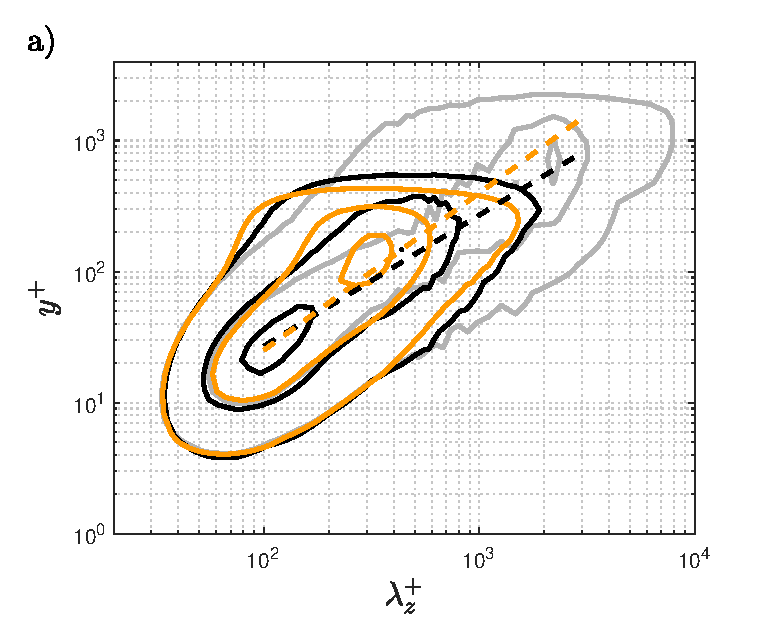
\includegraphics[width=0.49\textwidth]{fig12a.eps}
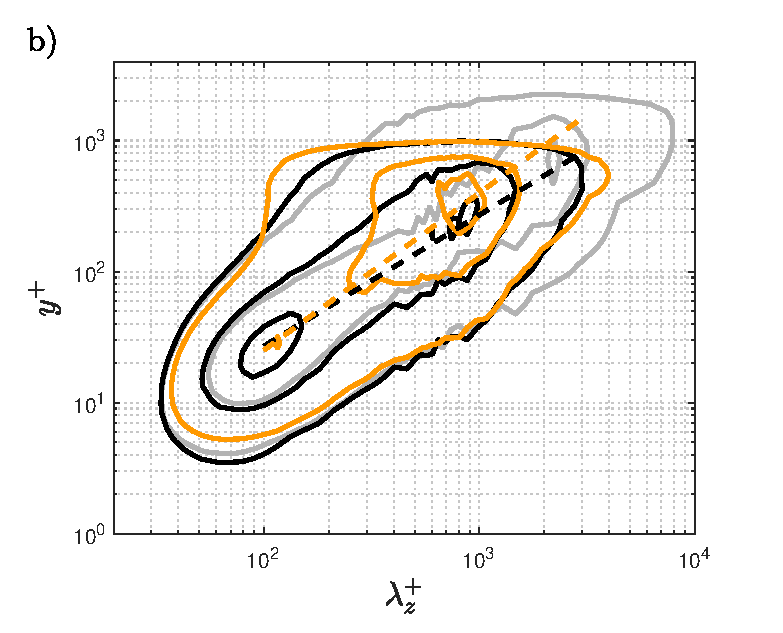
\includegraphics[width=0.49\textwidth]{fig12b.eps}
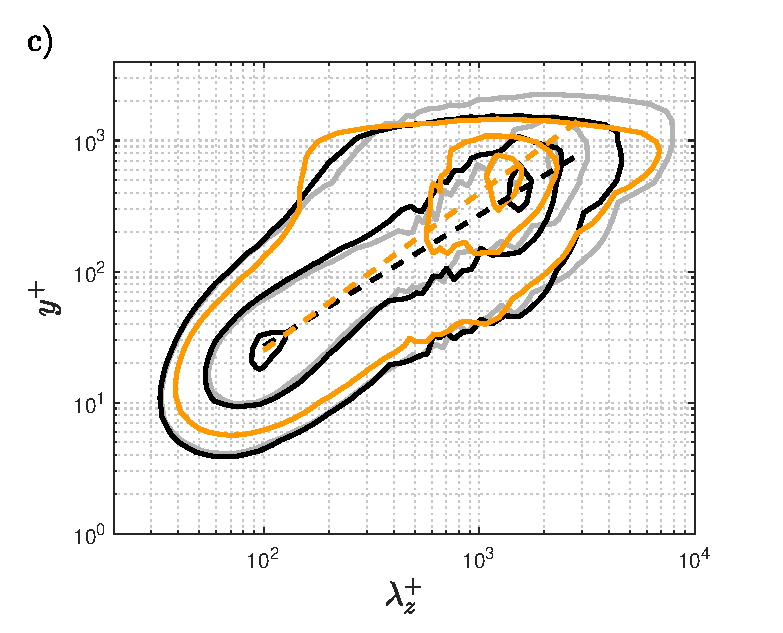
\includegraphics[width=0.49\textwidth]{fig12c.eps}
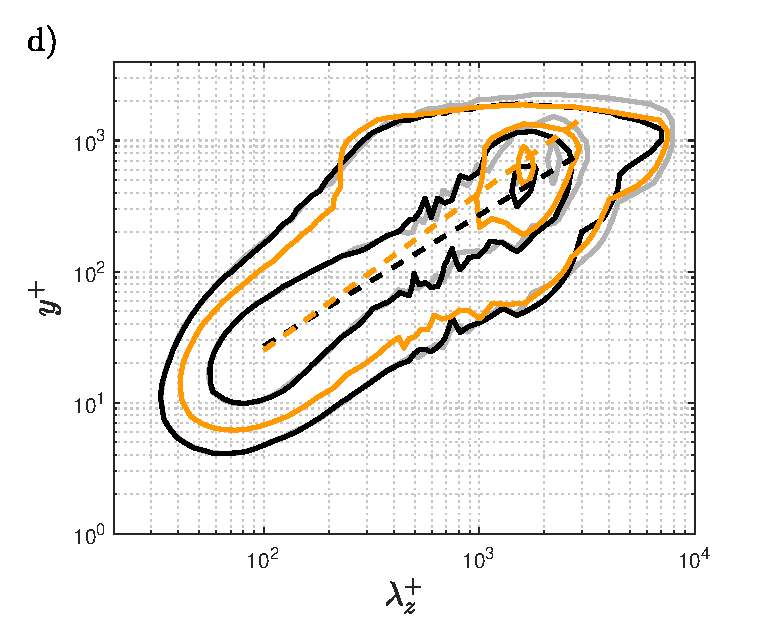
\includegraphics[width=0.49\textwidth]{fig12d.eps}
  \caption{ Premultiplied cospectra $k_z |\phi_{uv}|$ scaled with the local maximum for the b1.4 and ZPG cases at matched $\Rey_{\tau}$. Contours taken at $10\%$, $50\%$, $90\%$ of the maximum value. Reference contour in gray colour: ZPG at $Re_{\tau}=2386$. Dashed black lines show the curve $y^+=0.27 \lambda_z^+$ as in \cite{giovanetti2016}, while the orange dashed lines represent $y^+=0.1 (\lambda_z^+)^{1.2}$, which is the ridge for the b1.4 case. Colors: (\protect\blackline) ZPG; (\protect\orangeline) b1.4. (Top-left) $Re_{\tau}=500$, (top-right) $Re_{\tau}=1000$, (bottom-left) $Re_{\tau}=1500$, (bottom-right) $Re_{\tau}=2000$.}
\label{fig:spec1DUV}
\end{figure}

In figure \ref{fig:spec1DUV} we show the premultiplied cospectra $k_z |\phi_{uv}|$ at the same matched $\Rey_{\tau}$ as in figure \ref{fig:spec1DUU}. 
At the lowest $\Rey_{\tau}$ the contours in the APG and the ZPG are similar, with the difference that the maximum value is in the outer region in the former ($y^+=120$ and $\lambda_z^+=307$) and closer to the wall ($y^+=26$ and $\lambda_z^+=109$) in the latter.
In the $10\%$ and $50\%$ contours, it is possible to see a small contribution of the small scales in the outer region compared to the ZPG contours.
At higher Reynolds numbers, the ZPG  develops a plateau of energy with contour levels following a straight line of slope $C$, which in a logarithmic plot corresponds to a power law of the form: $y^+=(\lambda_z^+)^C$.
This line connects the near-wall peak  with the outer region. Furthermore, the plateau indicates a progressive growth of the region containing this level of energy following the previous power law, which at $\Rey_{\tau}=1000$ develops an outer peak with a magnitude similar to that of the near-wall peak. Note that at higher Reynolds numbers the outer peak progressively rises over the magnitude of the near-wall peak.
The effect of the APG is to displace the near-wall energy to the outer region, which becomes dominant in the premultiplied cospectra of the Reynolds shear stress. At higher Reynolds numbers, the premultiplied cospectra exhibit a peak at $\lambda_z \simeq \delta_{99}$, which implies that this peak scales in outer units.
The constant $C$ which defines the slope of the black dashed lines in figure \ref{fig:spec1DUV} was reported to be $\approx 1$ by \cite{giovanetti2016}. The APG exhibits $10\%$ contours similar to those of the ZPG, indicating the presence of some energy in the near-wall region. If a line from the inner peak of the ZPG is drawn towards the APG peak in the outer region (orange dashed lines in figure \ref{fig:spec1DUV}), its slope is larger than that of the ZPG. If a self-similar hierarchy of motions in the log-layer is suggested by the black dashed line, in connection with the attached-eddy hypothesis \citep{Townsend_1976, deshpande_2021}, then the APG either rises the slope of that hierarchy of scales or follows the same hierarchy of motions as in the ZPG with an additional contribution in the outer region by small scales risen from the wall by the wall-normal convection of the APG and by the more energetic large scales.

The premultiplied spectra for the wall-normal fluctuations is shown in the first row of figure \ref{fig:spec1D_VV_WW}. It exhibits features similar to those of the cospectra of the Reynolds shear stress: small-scale energy in the outer region due to the APG and a different location of the maximum power-spectral density in the ZPG and the APG. While the ZPG exhibits an elongated $90\%$ contour around $\lambda_z^+ \approx 150$ at $y^+\approx 90$ for the different Reynolds numbers, the APG starts to stretch the peak at the lowest $\Rey_{\tau}=500$, and at $\Rey_{\tau}=1000$ the peak is located in the outer region with scales of the order of $\lambda_z \simeq \delta_{99}$.
In the ZPG the $10\%$ contours in the wall-normal spectra exhibit a shape similar to that of the $50\%$ contours in the cospectra. Approximating the $10\%$ contour by an ellipse, the major axis also follows a trend $y^+=(\lambda_z^+)^C$ with $C=1$, as in the cospectra. The $50\%$ contours also exhibit linear regions, but in the wall-normal spectra the slopes are different. This could still be related to a hierarchy of motions in the logarithmic layer, just indicating that the range of wall-normal scales grows with the wall-normal location and as before, the APG adds an extra contribution from the small and highly-energetic large scales in the outer part of the logarithmic layer. The $10\%$ contours of the APG follow the trend dictated by $\Rey_{\tau}$ and far from the trend marked by $y^+=(\lambda_z^+)^C$; for this reason, we have not included those linear trends.
As can be observed in the second row of figure \ref{fig:spec1D_VV_WW}, the spectra of the spanwise fluctuations exhibit effects similar to those shown in the wall-normal spectra in the first row for the ZPG and the APG. In particular we identify the small-scale contribution to the outer region and a stable $90\%$ contour for the ZPG expanding a long range of scales from $\lambda_z^+\approx 15$ to $\lambda_z^+\approx 70$ in a region between $y^+=15$ and $y^+=100$, which is inside the overlap region. This $90\%$ contour is displaced by the APG towards regions farther than $y^+=300$, already in the wake region. The $\lambda_z^+$ of this peak also scales with the Reynolds number.

\begin{figure}
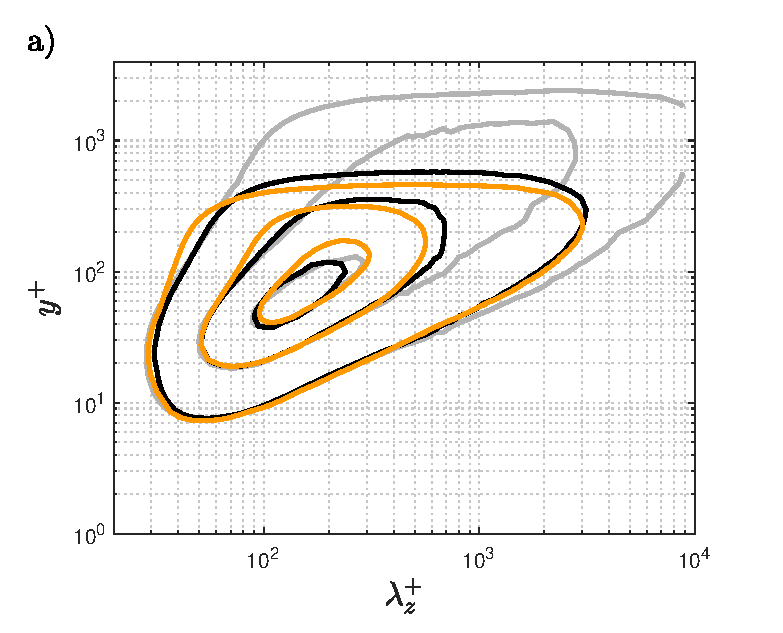
\includegraphics[width=0.245\textwidth]{fig13a.eps}
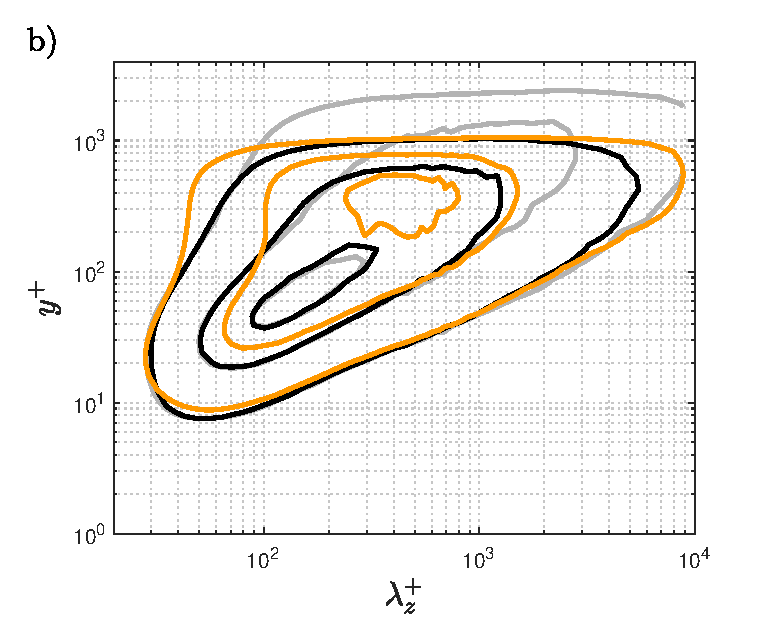
\includegraphics[width=0.245\textwidth]{fig13b.eps}
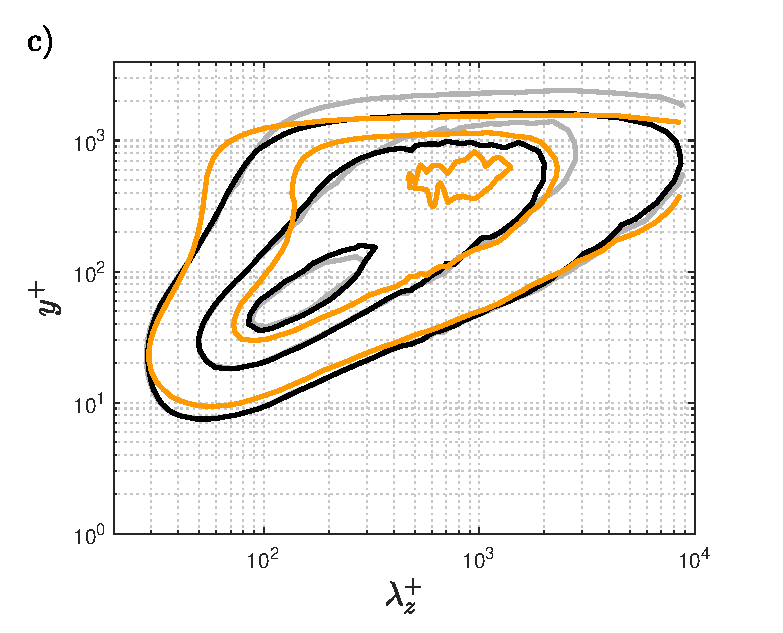
\includegraphics[width=0.245\textwidth]{fig13c.eps}
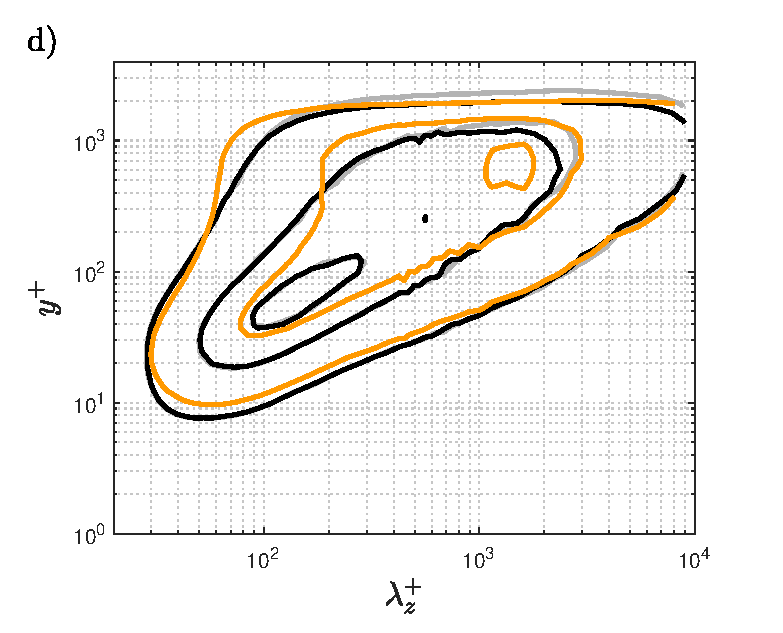
\includegraphics[width=0.245\textwidth]{fig13d.eps}
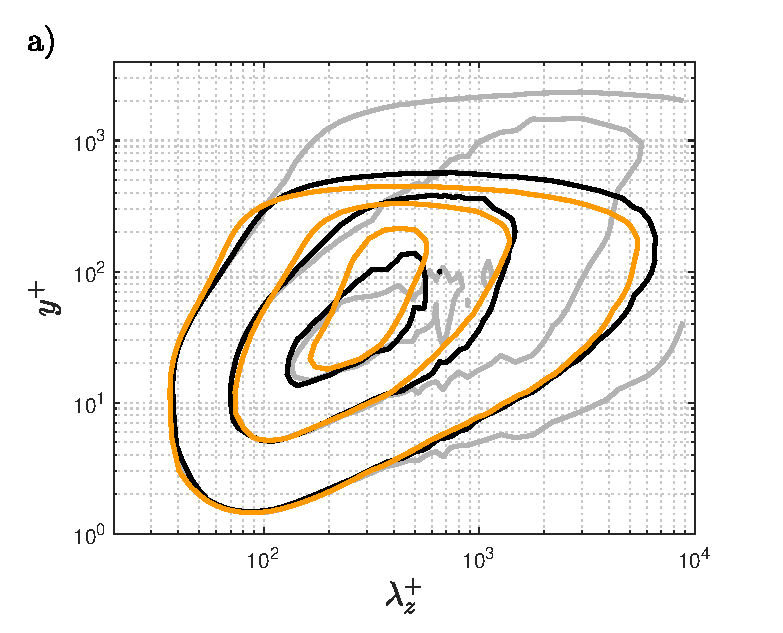
\includegraphics[width=0.245\textwidth]{fig13e.eps}
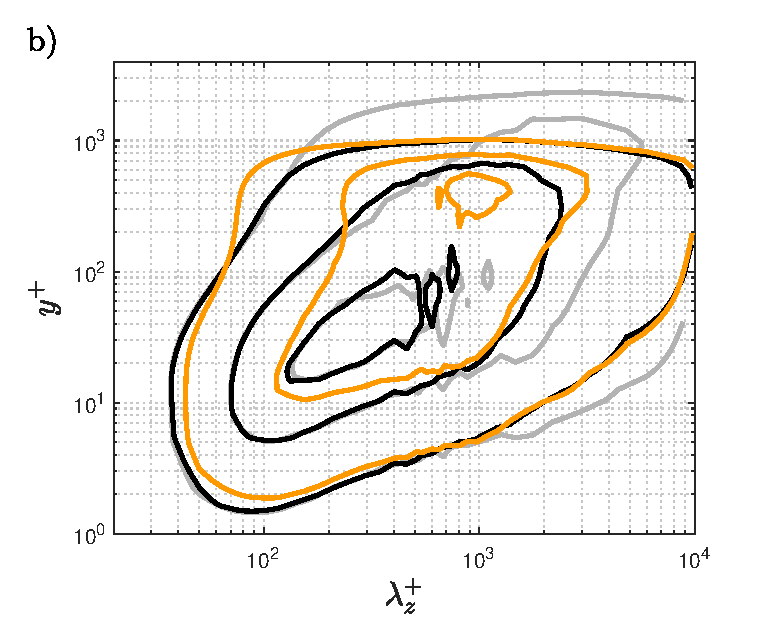
\includegraphics[width=0.245\textwidth]{fig13f.eps}
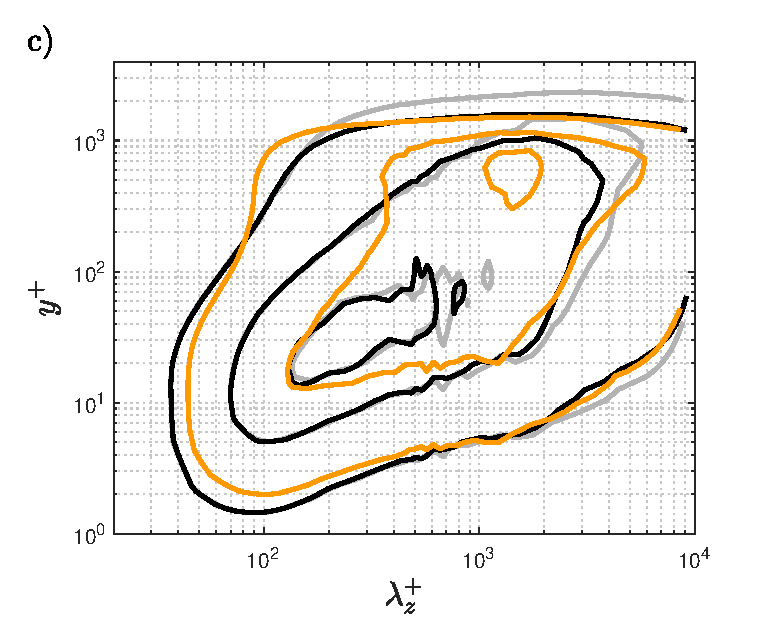
\includegraphics[width=0.245\textwidth]{fig13g.eps}
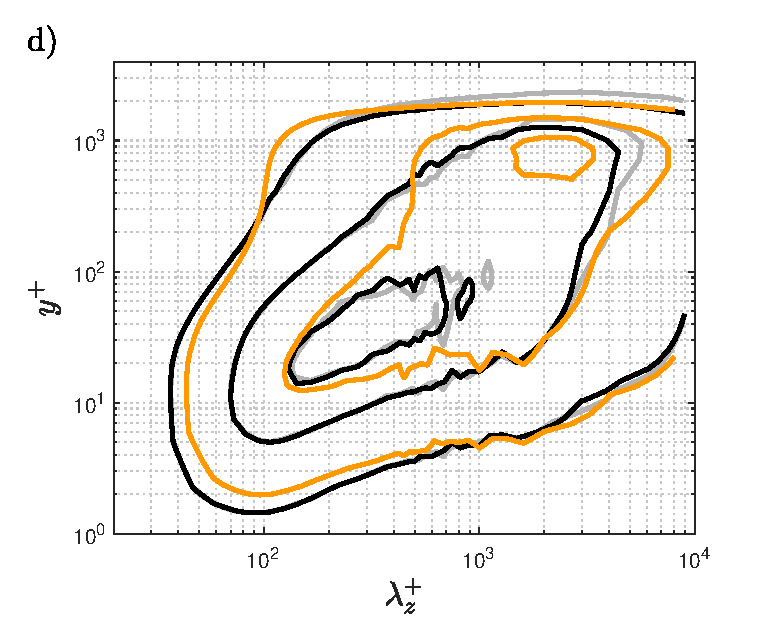
\includegraphics[width=0.245\textwidth]{fig13h.eps}
  \caption{Premultiplied spanwise power-spectral density of $k_z |\phi_{vv}|$ (first row) and $k_z |\phi_{ww}|$ (second row) scaled with the local maximum for the b1.4 and ZPG cases at matched $\Rey_{\tau}$. Contours taken at $10\%$, $50\%$, $90\%$ of the maximum value. Reference contour in gray colour: ZPG at $Re_{\tau}=2386$. Contours with (\protect\blackline) for ZPG and (\protect\orangeline) for b1.4. From left to right: $Re_{\tau}=500$, $Re_{\tau}=1000$, $Re_{\tau}=1500$ and $Re_{\tau}=2000$.}
\label{fig:spec1D_VV_WW}
\end{figure}

%-----------------Spectra 2D------------------------------------------------------------
%-----uu--------------------

\subsection{Two-dimensional power-spectral density}

The two-dimensional power-spectral energy $E_{u_iu_j}(k_z,k_t,y)$ is obtained using temporal series of the velocities in all the spanwise grid points at selected streamwise and wall-normal positions. Once the mean in time and spanwise direction is substracted, the turbulent components are transformed to Fourier space in the spanwise wavenumbers. To obtain the power spectra in time, Welch's method is used with 8 independent subdivisions in time overlapped with 7 subdivisions for a total of 15 bins. The window function is a Hamming window.
The spectral energy is then divided by $\Delta k_z \Delta k_t$ to obtain the two-dimensional power-spectral density $\phi(k_z,k_t,y)$. As above, the figures used to illustrate the effects of the Reynolds number and the APG in the spectral-density content will be premultiplied, in this case, with the factor $k_z k_t$.
It has been verified that the addition of the spectral energy for all the wavenumbers in time yields the one-dimensional power-spectral energy in the spanwise direction $E_{u_i u_j}(k_z,y)$.


\subsubsection{Two-dimensional power-spectral density in the near-wall region}

The premultiplied power-spectral density in time and the spanwise direction $k_zk_t\phi(\lambda_z, \lambda_t)$ is first analysed at $y^+=15$, a wall-normal location which shows the characteristics of the near-wall peak of the streamwise RS and the production of TKE.
\begin{figure}
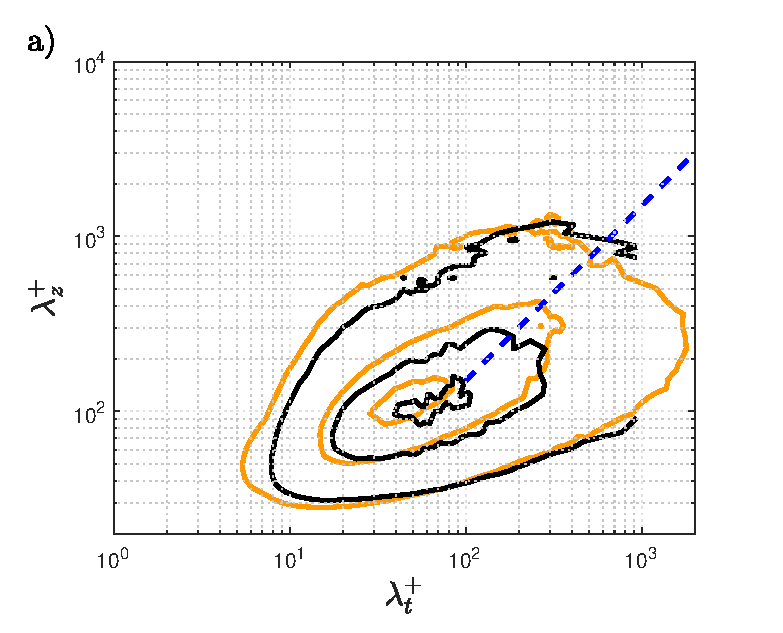
\includegraphics[width=0.24\textwidth]{fig14a.eps}
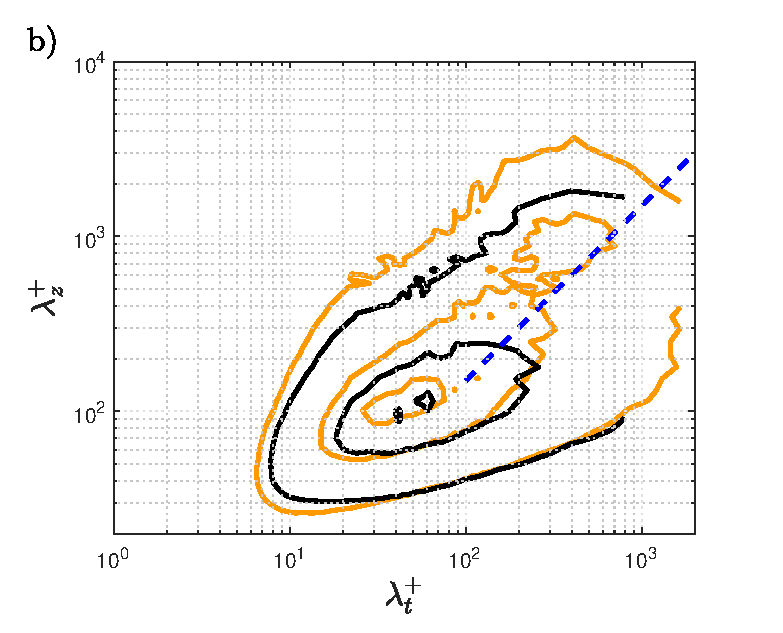
\includegraphics[width=0.24\textwidth]{fig14b.eps}
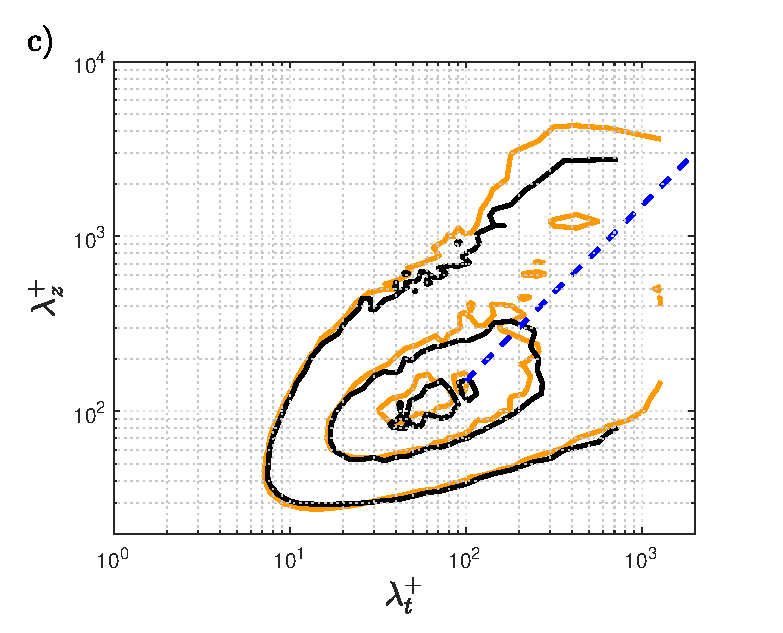
\includegraphics[width=0.24\textwidth]{fig14c.eps}
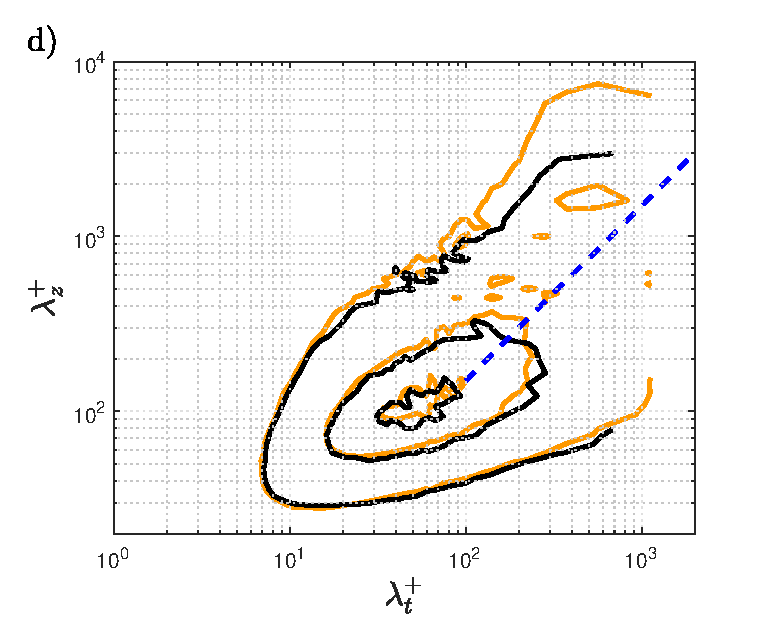
\includegraphics[width=0.24\textwidth]{fig14d.eps}
  \caption{Two-dimensional premultiplied power-spectral density $k_z k_t |\phi_{uu}|$ at $y^+=15$ scaled with the local maximum. Contours taken at $10\%$, $50\%$, $90\%$ of the maximum value. From left to right: $Re_{\tau}=500$, $Re_{\tau}=1000$, $Re_{\tau}=1500$ and $Re_{\tau}=2000$. The dashed blue line represents $\lambda_z^+ = 1.5\lambda_t^+$. Contours with (\protect\blackline) for ZPG and (\protect\orangeline) for b1.4.}
\label{fig:spec2D_uu_y15}
\end{figure}
For all the Reynolds numbers shown in figure \ref{fig:spec2D_uu_y15} there is a near-wall spectral peak with $\lambda_z^+ \approx 100$ and $\lambda_t^+$ of the order of 100. The blue dashed line represents $\lambda_z^+ = 1.5\lambda_t^+$, which describes the evolution with $\Rey$ of the ridge in the upper-right part of the spectrum. This ridge was documented by \cite{Hoyas_PoF2006} for channels, \cite{Sillero_2011}, for ZPG TBLs and \cite{tanarro_2020} for APG TBLs.
The APG does not significantly modify the spectrum around the near-wall peak and the local viscous length and time scales $l_{\tau}$ and $t_{\tau}$ lead to the collapse of the inner region for the three displayed contour levels.
Some extra energy is seen in the APG with the $50\%$ contours in the region with larger $\lambda_z^+$ and $\lambda_t^+$.
The biggest difference in the inner region is seen for the lowest Reynolds number, which is upstream of the ROI where near-equilibrium is achieved. At higher $\Rey_{\tau}$ values of 1000, 1500 and 2000, the spectra around the near-wall peak are identical for each simulation and grow closer to the ZPG contours. In figure \ref{fig:spec2D_uiuj_y15}, only the contours at $\Rey_{\tau}=500$ and 2000 are represented to show the differences in the region around the near-wall peak due to $\Rey_{\tau}=500$ being outside of the near-equilibrium region and to show the growth of the largest spatio-temporal scales.
\begin{figure}
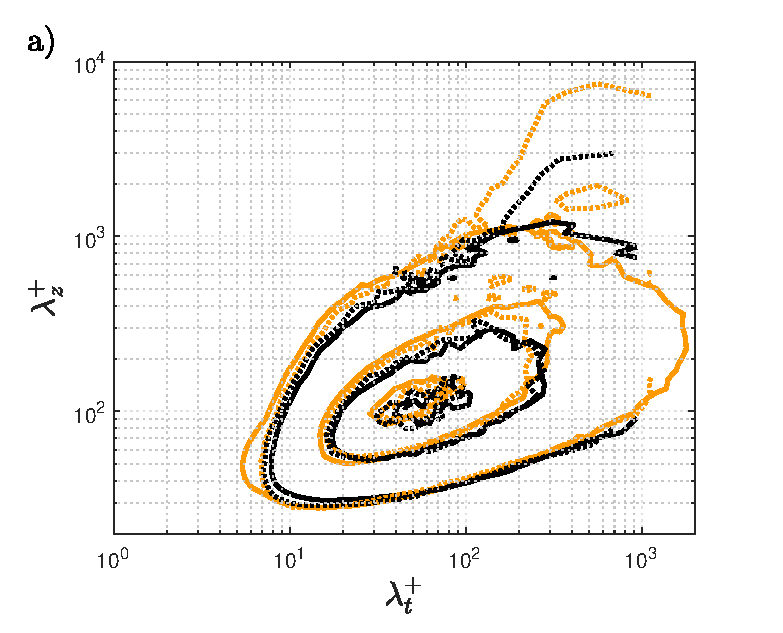
\includegraphics[width=0.49\textwidth]{fig15a.eps}
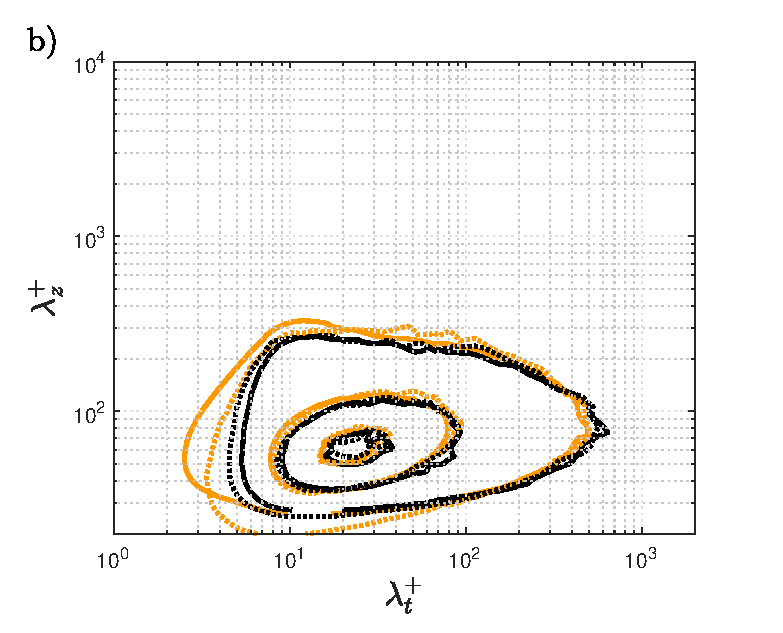
\includegraphics[width=0.49\textwidth]{fig15b.eps}
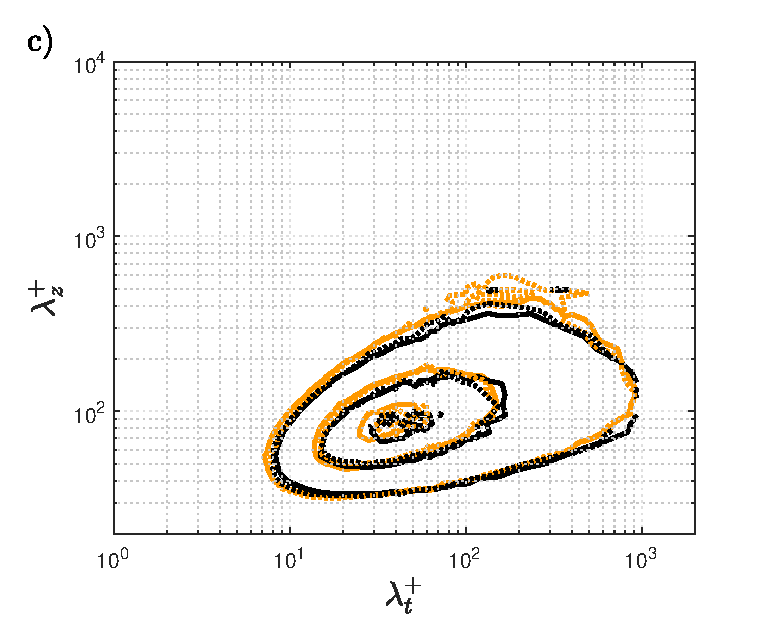
\includegraphics[width=0.49\textwidth]{fig15c.eps}
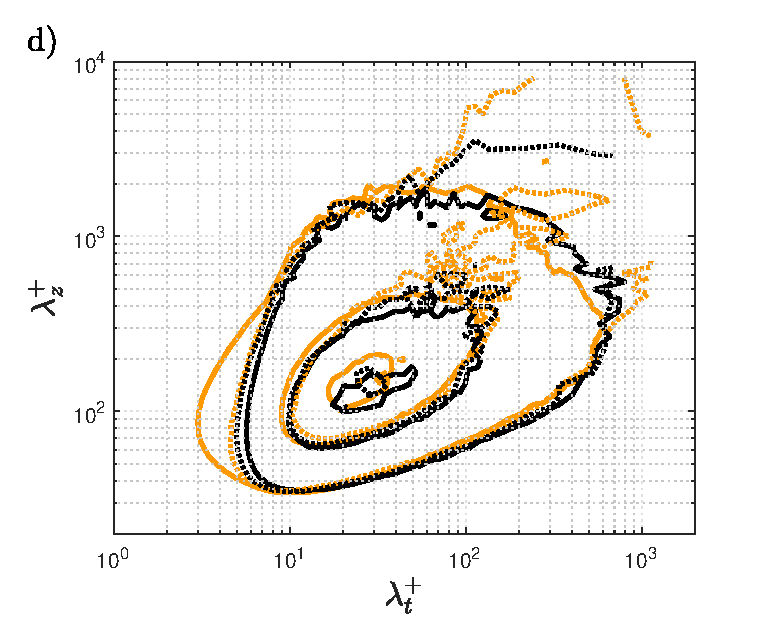
\includegraphics[width=0.49\textwidth]{fig15d.eps}
  \caption{Evolution with the Reynolds number of the two-dimensional premultiplied power-spectral density in time and $z$ for the various Reynolds-stress components $k_z k_t |\phi_{u_iu_j}|$ at $y^+=15$ scaled with the local maximum. The panels show spectra of: a) $uu$, b) $vv$, c) $uv$, d) $ww$. Contours taken at $10\%$, $50\%$, $90\%$ of the maximum value. Solid lines for $Re_{\tau}=500$ and dotted lines for $Re_{\tau}=2000$. Colors: (\protect\blackline) for ZPG and (\protect\orangeline) for b1.4.}
\label{fig:spec2D_uiuj_y15}
\end{figure}

Surprisingly, the cospectra of the Reynolds shear stress shown in figure \ref{fig:spec2D_uiuj_y15}c) at $y^+=15$ does not exhibit significant differences between APG and ZPG nor with increasing $\Rey_{\tau}$. 
The behaviour of the streamwise and spanwise components is similar, since at higher Reynolds numbers the ZPG and the APG contours grow closer, both developing a region with larger values of $\lambda_z^+$, $\lambda_t^+$ with a higher energy content.
The wall-normal Reynolds stress does not develop a region with larger scales, and the lowest-density contour grows in the direction of smaller $\lambda_z^+$, $\lambda_t^+$.
The effect of $\Rey_{\tau}=500$ not being in near-equilibrium, as opposed to the higher-$\Rey_{\tau}$ profiles at 1000, 1500 and 2000 is reflected in a different slope of the $10\%$ contour in the lower region of the premultiplied spectra for the normal Reynolds stresses.


\subsubsection{Two-dimensional power-spectral density in the overlap region}
The analysis for the overlap region will be done at $y^+=150$ as in \cite{tanarro_2020} to compare the trends of $\lambda_{z}^+=f(\lambda_{t}^+)$ previously reported for channel flows in \cite{delAlamo_jfm_2004} and for boundary layers in \cite{chandran_jfm_rapids_2017}.
\begin{figure}
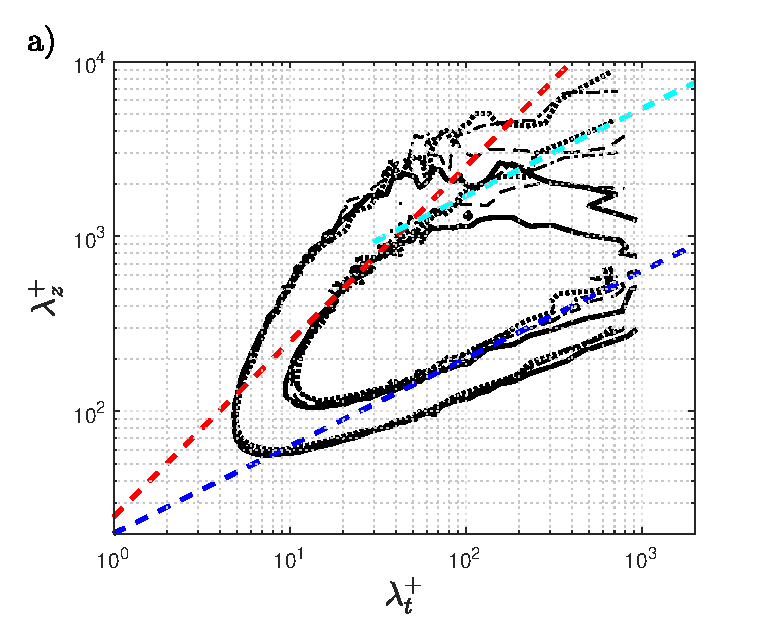
\includegraphics[width=0.31\textwidth]{fig16a.eps}
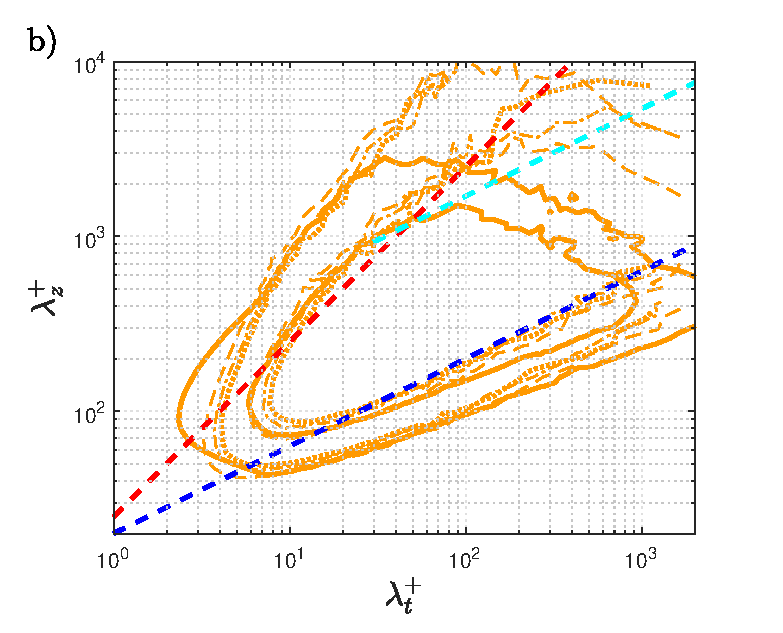
\includegraphics[width=0.31\textwidth]{fig16b.eps}
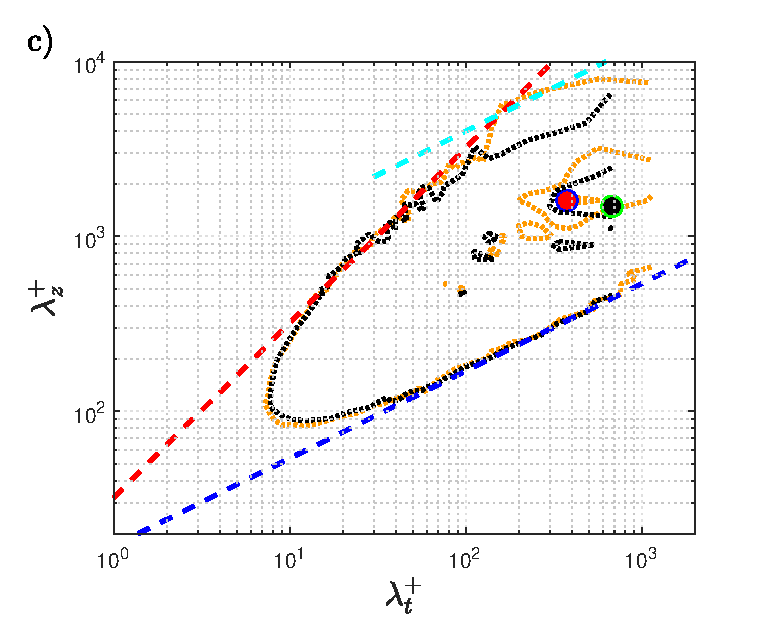
\includegraphics[width=0.31\textwidth]{fig16c.eps}
  \caption{Two-dimensional premultiplied power-spectral density $k_z k_t |\phi_{uu}|$ at $y^+=150$. The line styles solid, dashed, dash-dotted and dotted correspond to $Re_{\tau}=500, 1000, 1500$ and 2000 respectively. a) and b) are scaled with inner units, $u_{\tau}^2$, and show the contour levels 0.05 and 0.15 of the ZPG and b1.4 respectively. In a) and b) the red, blue and cyan lines are tangent to the contour level 0.15 of the ZPG. c) Represents both ZPG and b1.4 scaled with the local maximum marked as a black dot for ZPG and as a red dot for b1.4. The contours are taken at $10\%$ and $50\%$ of the maximum value. In c) the red, blue and cyan lines are moved to be tangent to the $10\%$ contour. Blue and cyan lines follow $\lambda_z^+ \propto (\lambda_t ^{+})^{0.5} $, while red line represents $\lambda_z^+ \propto \lambda_t^+$. Colors: (\protect\blackline) for ZPG and (\protect\orangeline) for b1.4.}
\label{fig:spec2Duu_yp150}
\end{figure}
In figure \ref{fig:spec2Duu_yp150} we show for $y^+=150$ the contour levels of energy 0.05 and 0.15 for the ZPG and for b1.4. At this wall-normal location and for the energy level 0.15, it was reported in \cite{tanarro_2020} a lower bound for small time and spanwise scales following $\lambda_z^+ \propto (\lambda_t ^{+})^{0.5} $ (blue-dashed line) and an upper bound composed by the red-dashed line ($\lambda_z^+ \propto \lambda_t^+$) for shorter time scales, as well as the cyan-dashed line for longer time scales (same slope as the blue-dashed line).
For the ZPG it is possible to see that for short scales there is a good collapse for different Reynolds numbers, and the lower limit (blue line) serves as a good approximation in spite of a small tendency with higher Reynolds numbers (at higher $\lambda_t^+$) to go towards wider scales for the same time scale.
The lower-energetic level 0.05 also presents a good collapse for the different Reynolds numbers, however, the slope of the trend (0.4) is slightly smaller than the one for energy level 0.15 (0.5).
The upper part of the contours are more curved than the lower part, therefore it is harder to come up with a linear trend in a logarithmic plot (potential law). The red line approximates a short region, $\lambda_t^+ \in (20, 60)$, while the cyan line seems to be a good approximation for the larger scales at higher Reynolds numbers.
The tangent lines to the energetic contour 0.15 of the ZPG are presented also in figure \ref{fig:spec2Duu_yp150}b) as a way to compare with the same energetic contour in b1.4. It is clear that in inner-scaling, the same energy contour is bigger in the APG than in the ZPG, expanding over shorter and larger scales. There is also a bigger dispersion of the contours due to the increasing Reynolds numbers.
The lower limits exhibit a slightly different slope than the blue line, however, with an increasing Reynolds number (dotted orange line) the trend is closer to the blue-dashed line. Since this is a fixed location at $y^+=150$ (see figure \ref{fig:spec1DUU}) at higher Reynolds numbers the differences between APG and ZPG are shifted towards higher wall-normal positions and larger $\lambda_z^+$ scales.
The red line ($\lambda_z^+ \propto \lambda_t^+$) appears to be a better approximation for the upper limit that will expand over a longer region , {\it i.e.} $\lambda_t^+ \in (10, 200)$ for $\Rey_{\tau}=2000$ compared to the case of the ZPG. The cyan line also seems to be a good approximation for the larger scales.
For $\Rey_{\tau}=2000$ the location of the local maximum for APG and ZPG is very similar. If the power-spectral density is non-dimensionalized by the local maximum as in figure \ref{fig:spec2Duu_yp150}c) the $10\%$ and $50\%$ contours of the ZPG and APG cases appears to collapse, except for some extra energy in the APG in the largest $\lambda_z^+$ and $\lambda_t^+$. The trends marked by the blue, red and cyan dashed lines are a better approximation at the higher $\Rey$.

For the lowest $\Rey_{\tau}$ in figure \ref{fig:spec2Duu_yp150_max} there is not a clear separation of scales. For each wall-normal plane, the local maximum of $k_z k_t |\phi_{uu}|$ evolves from the characteristic inner-peak wavelengths of $\lambda_z^+=100$ at $y^+=15$ towards wider scales $\lambda_z$ of the order of $\delta_{99}$ in the outer region.
At a higher Reynolds number as $\Rey_{\tau}=1000$ the location of the maxima in these premultiplied plots changes radically from scales $\lambda_z^+ \approx \mathcal{O} (100)$ and $\lambda_t^+ \approx \mathcal{O} (\lambda_z^+/2)$ to scales $\lambda_z \approx \mathcal{O}(\delta_{99})$. This change appears at $y^+\approx 23$ for b1.4 and $y^+\approx 40$ for the ZPG.  

At the position $y^+=150$ the peak of $k_z k_t |\phi_{uu}(k_z,k_t)|$ is already in scales $\lambda_z \approx \delta_{99}$ as it can be seen in figure \ref{fig:spec2Duu_yp150_max}c).
The other components of the Reynolds stress tensor are shown in figure \ref{fig:spec2Duiuj_150}.
As it was seen near the wall, at the lowest $\Rey_{\tau}=500$ (solid lines), the $10\%$ contour shows an additional content of energy for b1.4 in the smaller $\lambda_z^+$ scales with lower $\lambda_t^+$. 
The APG effects are manifested as a deviation of the local peak position and as it was seen near the wall, in the presence of small scales with shorter $\lambda_t^+$ in the wall-normal component, see figure \ref{fig:spec2Duiuj_150}b).
Previously, near the wall, the spectra containing wall-normal velocities in figure \ref{fig:spec2Duiuj_150}b) and c) was practically unaffected by an increase in the Reynolds number. On the other hand, in the outer region, both components develop larger spatio-temporal scales when the Reynolds number is increased. 
As observed in figure \ref{fig:spec2Duu_yp150_max}d) (and also in figure \ref{fig:spec2Duu_yp150}c)), the red-dashed line which approximates the contours for scales up to $\lambda_t^+ =100$ in the ZPG, reaches scales up to $\lambda_t^+ =200$ in the APG \citep{chandran_jfm_rapids_2017}.
The extra energy in the small scales with lower $\lambda_t^+$ is only seen in the lower $\Rey_{\tau}=500$ profiles of b1.4; for $\Rey_{\tau}=1000$, 1500 and 2000 that region is exhibits collapse.
In the 2D spectra shown in \cite{tanarro_2020}, the profiles were taken at different levels of the premultiplied spectral density scaled either in viscous or outer units. They reported that at the same contour level the APG effects extend over a wider range of scales compared to the ZPG contours at the same low $\Rey_{\tau}=305$. However, note that in their case the Reynolds number was low, the APG very strong and their boundary layers were not in near-equilibrium, exhibiting a rapid change in the $\beta(x)$ curve. Even if they achieved a value of $\beta$ larger than in the b1.4 simulation and an increase of the energy in the outer regions of the $\overline{u^2}^+$ TKE production profiles, the separation of scales in their study was not enough to observe the effects exhibited by the b1.4 simulation.

\begin{figure}
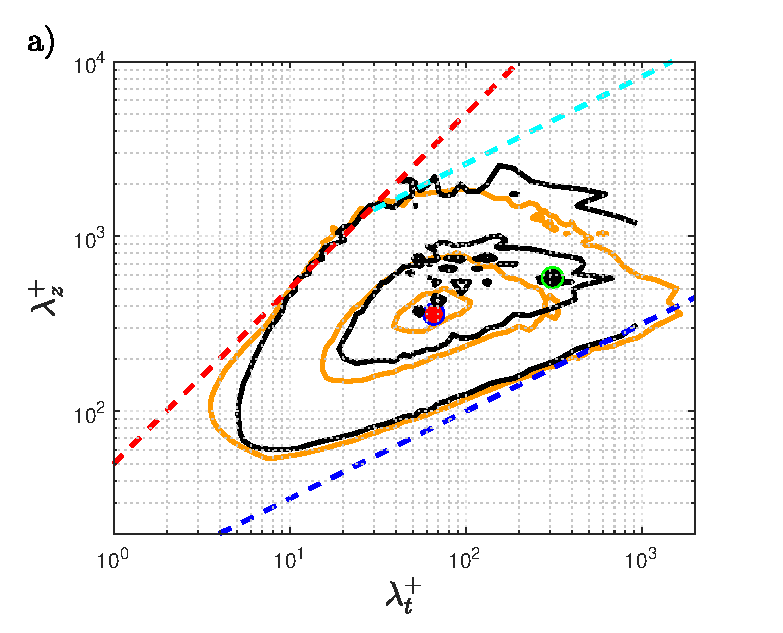
\includegraphics[width=0.49\textwidth]{fig17a.eps}
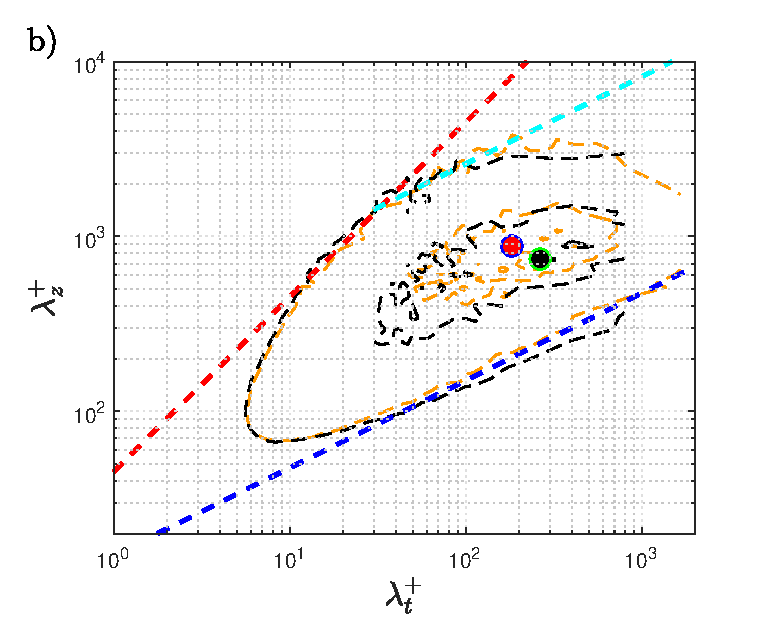
\includegraphics[width=0.49\textwidth]{fig17b.eps}
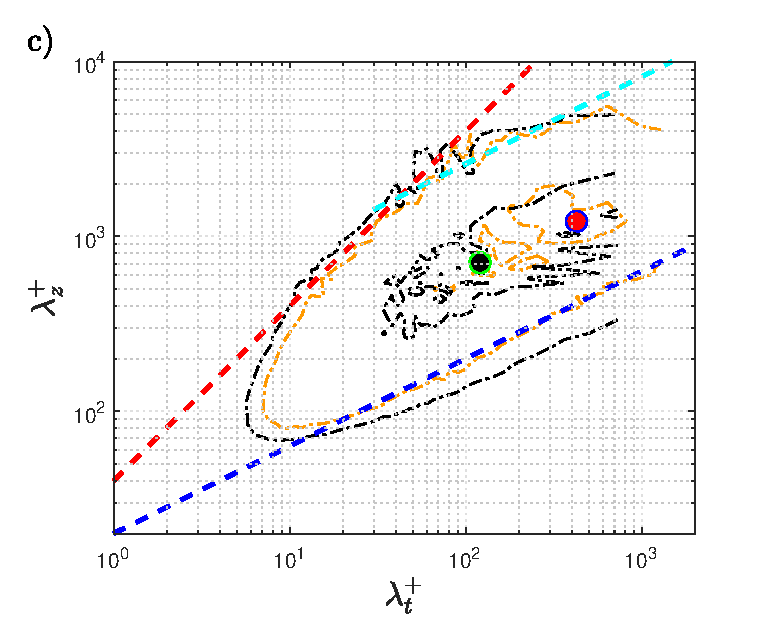
\includegraphics[width=0.49\textwidth]{fig17c.eps}
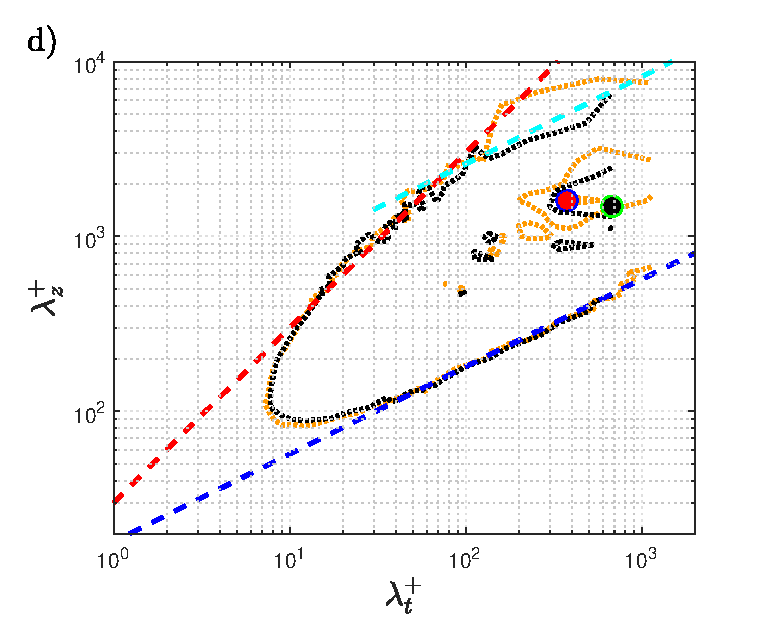
\includegraphics[width=0.49\textwidth]{fig17d.eps}
  \caption{Two-dimensional premultiplied power-spectral density $k_z k_t |\phi_{uu}|$ at $y^+=150$ scaled with the local maximum. Contours taken at $10\%$, $50\%$, $90\%$ of the maximum value. From left to right: a) $Re_{\tau}=500$, b) $Re_{\tau}=1000$, c) $Re_{\tau}=1500$ and d) $Re_{\tau}=2000$. The dashed blue and cyan lines represent $\lambda_z^+ \approx (\lambda_t^+)^{1/2}$, the dashed red line represents $\lambda_z^+ \approx \lambda_t^+$. The red and black dots mark the position of the local maximum for b1.4 and ZPG respectively. Colors: (\protect\blackline) for ZPG and (\protect\orangeline) for b1.4.}
\label{fig:spec2Duu_yp150_max}
\end{figure}

\begin{figure}
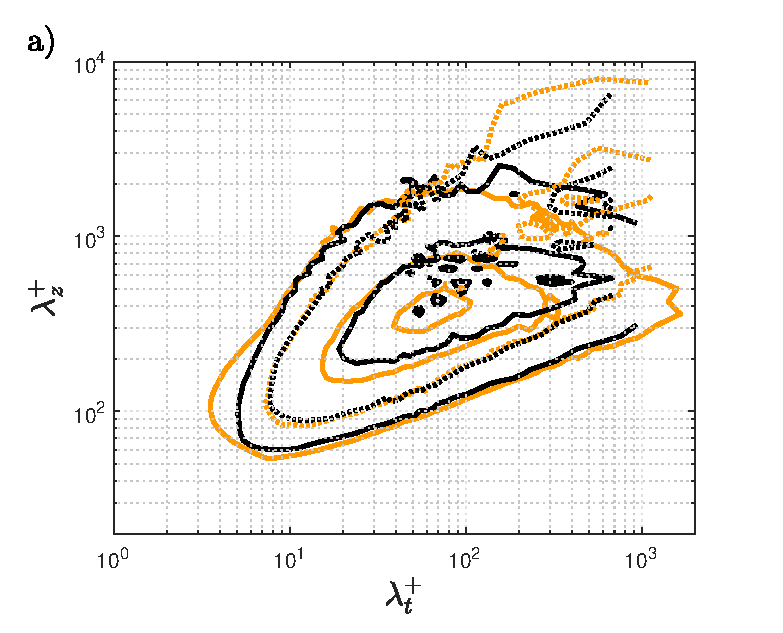
\includegraphics[width=0.49\textwidth]{fig18a.eps}
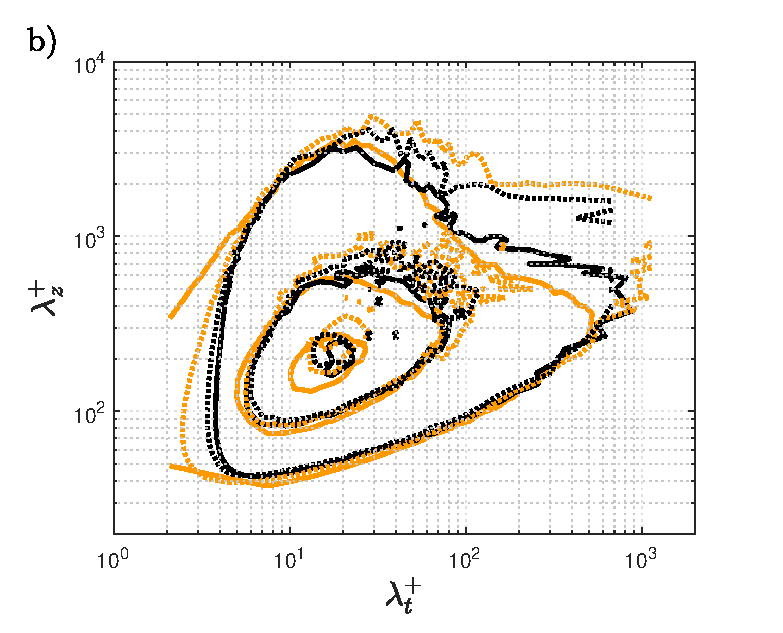
\includegraphics[width=0.49\textwidth]{fig18b.eps}
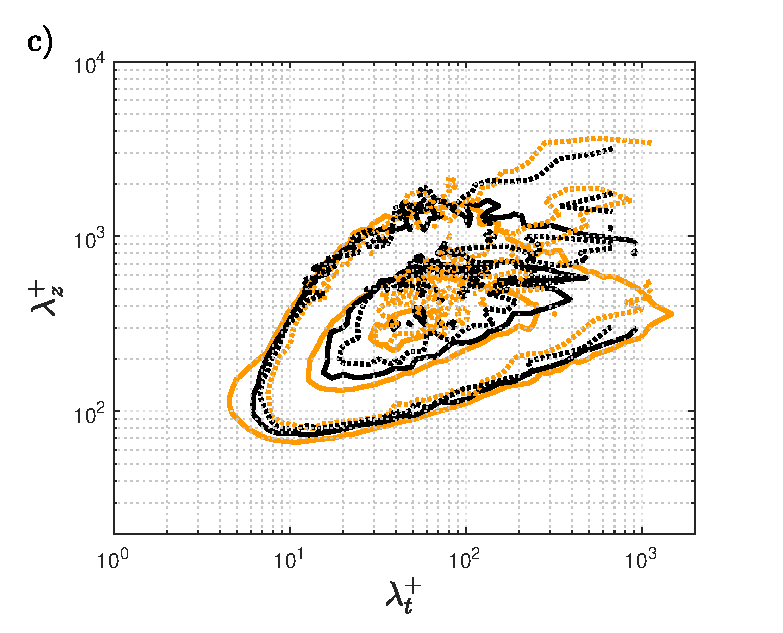
\includegraphics[width=0.49\textwidth]{fig18c.eps}
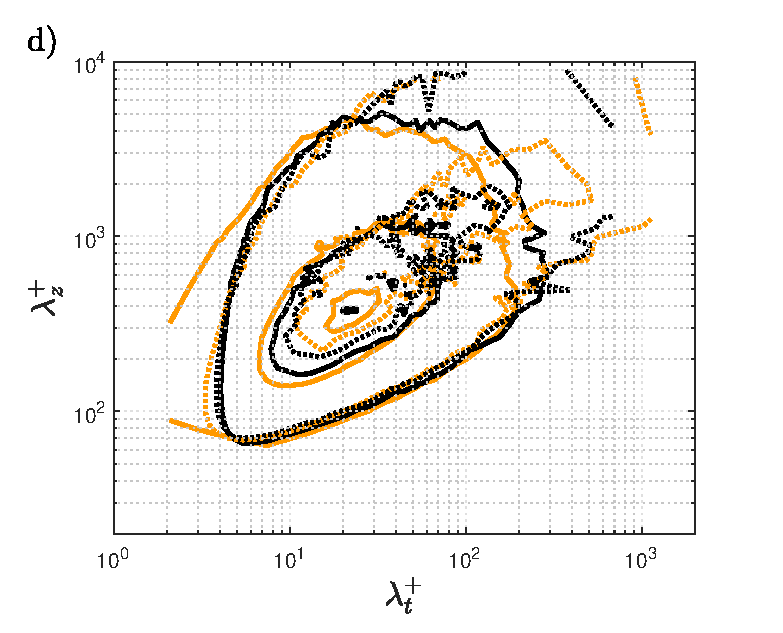
\includegraphics[width=0.49\textwidth]{fig18d.eps}
  \caption{Evolution with the Reynolds number of the two-dimensional premultiplied power-spectral density of the Reynolds-stress components $k_z k_t |\phi_{u_iu_j}|$ at $y^+=150$ scaled with the local maximum. The panels show spectra of: a) $uu$, b) $vv$, c) $uv$, d) $ww$. Contours taken at $10\%$, $50\%$, $90\%$ of the maximum value. Solid lines for $Re_{\tau}=500$ and dotted lines for $Re_{\tau}=2000$. Colors: (\protect\blackline) for ZPG and (\protect\orangeline) for b1.4.}
\label{fig:spec2Duiuj_150}
\end{figure}

